
%(BEGIN_QUESTION)
% Copyright 2013, Tony R. Kuphaldt, released under the Creative Commons Attribution License (v 1.0)
% This means you may do almost anything with this work of mine, so long as you give me proper credit

Examine this natural gas compressor system with inlet separator vessel:

$$\includegraphics[width=15.5cm]{i0003rx01.eps}$$

Examine this P\&ID and answer the following questions:

\begin{itemize}
\item{} Why is it important that the separator vessel be placed upstream of the compressor?  Why not place it on the discharge side of the compressor instead?
\vskip 10pt
\item{} What might cause the compressor to vibrate excessively, thus requiring a vibration monitoring system?
\vskip 10pt
\item{} What effect will opening the recycle valve (XV-76) have on the effective {\it compression ratio} of this compressor as it is operating?
\vskip 10pt
\item{} What measured variables in this system might indicate that the compressor is being overloaded (i.e. working too hard as it tries to compress more natural gas than it safely can)?
\end{itemize}

\underbar{file i04793}
%(END_QUESTION)





%(BEGIN_ANSWER)

\begin{itemize}
\item{} Why is it important that the separator vessel be placed upstream of the compressor?  Why not place it on the discharge side of the compressor instead?  {\it Liquids are incompressible, and so the purpose of the upstream separator vessel is to capture any entrained liquid droplets condense before they would have any chance of entering the compressor.}
\vskip 10pt
\item{} What might cause the compressor to vibrate excessively, thus requiring a vibration monitoring system?  {\it Any damage or wear to the compressor's rotating pieces causing it to become imbalanced.}
\vskip 10pt
\item{} What effect will opening the recycle valve (XV-76) have on the effective {\it compression ratio} of this compressor as it is operating? {\it Recycling gas through the compressor will reduce the net flow in this natural gas system as well as reduce the amount of differential pressure across the compressor.  Both of these effects will reduce the effective compression ratio of the compressor.} 
\vskip 10pt
\item{} What measured variables in this system might indicate that the compressor is being overloaded (i.e. working too hard as it tries to compress more natural gas than it safely can)?  {\it Excessive differential pressure (sensed by PDT-77), excessive discharge temperature (sensed by TT-232), excessive electrical power drawn by the compressor's motor (sensed by JT-220).}
\end{itemize}


%(END_ANSWER)





%(BEGIN_NOTES)


%INDEX% Process: gas compressor inlet separator (realistic P&ID shown)

%(END_NOTES)


